\documentclass[10pt,a4paper]{article}
\usepackage[utf8]{inputenc}
\usepackage[francais]{babel}
\usepackage[T1]{fontenc}
\usepackage{amsmath}
\usepackage{amsfonts}
\usepackage{amssymb}
\usepackage{graphicx}
\usepackage{enumitem}
\usepackage{lmodern}
\usepackage{listings}
\usepackage{color}

\definecolor{mygreen}{rgb}{0,0.6,0}
\definecolor{mygray}{rgb}{0.5,0.5,0.5}
\definecolor{mymauve}{rgb}{0.58,0,0.82}

\lstset{ %
  backgroundcolor=\color{white},   % choose the background color; you must add \usepackage{color} or \usepackage{xcolor}
  basicstyle=\footnotesize,        % the size of the fonts that are used for the code
  breakatwhitespace=false,         % sets if automatic breaks should only happen at whitespace
  breaklines=true,                 % sets automatic line breaking
  captionpos=b,                    % sets the caption-position to bottom
  commentstyle=\color{mygreen},    % comment style
  deletekeywords={...},            % if you want to delete keywords from the given language
  escapeinside={\%*}{*)},          % if you want to add LaTeX within your code
  extendedchars=true,              % lets you use non-ASCII characters; for 8-bits encodings only, does not work with UTF-8
  frame=single,                    % adds a frame around the code
  keepspaces=true,                 % keeps spaces in text, useful for keeping indentation of code (possibly needs columns=flexible)
  keywordstyle=\color{blue},       % keyword style
  language=Java,                 % the language of the code
  morekeywords={*,...},            % if you want to add more keywords to the set
  numbers=left,                    % where to put the line-numbers; possible values are (none, left, right)
  numbersep=5pt,                   % how far the line-numbers are from the code
  numberstyle=\tiny\color{mygray}, % the style that is used for the line-numbers
  rulecolor=\color{black},         % if not set, the frame-color may be changed on line-breaks within not-black text (e.g. comments (green here))
  showspaces=false,                % show spaces everywhere adding particular underscores; it overrides 'showstringspaces'
  showstringspaces=false,          % underline spaces within strings only
  showtabs=false,                  % show tabs within strings adding particular underscores
  stepnumber=2,                    % the step between two line-numbers. If it's 1, each line will be numbered
  stringstyle=\color{mymauve},     % string literal style
  tabsize=2,                       % sets default tabsize to 2 spaces
  title=\lstname                   % show the filename of files included with \lstinputlisting; also try caption instead of title
}
\usepackage[left=2cm,right=2cm,top=2cm,bottom=2cm]{geometry}


\date{24 octobre 2014}
\author{Groupe 2.2}
\title{Produit Mission 3}

\begin{document}
\maketitle

\section*{Question 1 : Arnaud Dethise}

	Les \texttt{Maps} sont des tableaux associatifs. Il s'agit d'un ensemble d'\textit{entries} qui sont des paires clé/valeur. Chaque entry associe une clé unique à sa valeur.

	Les méthodes principales sont \texttt{put(k,v)} qui ajoute à la map la valeur \textit{v} associé à la clé \textit{k} ; \texttt{get(k)} qui retourne la valeur associée à la clé \textit{k} ; et \texttt{remove(k)} qui retire l'entry donc la clé est \textit{k}.
	
	\vspace{0.35cm}

	Bien qu'il soit normalement possible de mettre un \texttt{null} comme valeur d'une entrée, certaines implémentations de Map en Java l'interdisent explicitement pour éviter les ambiguïtés dans le cas où une clé n'existe pas. En effet, si la clé \textit{k} n'existe pas, \texttt{get(k)} renverra \texttt{null}. Si une entrée (k,\texttt{null}) existe, \texttt{get(k)} renverra \texttt{null} non parce que la clé n'existe pas, mais parce que \texttt{null} est la valeur associée à \textit{k}.
	
	\vspace{0.35cm}
	
	Exemples d'applications importantes :
	\begin{itemize}
		\item Liste de membre de personnel. Par exemple, l'UCL avec une map, une entry par étudiant, le NOMA comme clé et le nom comme valeur.	
		\item Un DNS mappe une url avec l'ip qui lui est associée.
		\item Un programme de graphisme peut associer un alias (\texttt{bleu}) avec une couleur (\texttt{rgb(0,0,255)}).
	\end{itemize}

\section*{Question 2 : Arnaud Dethise}

	\subsection*{Hash table}
	
	Au lieu d'utiliser directement les objets comme clé, on calcule leur hash code qui est ensuite compressé en un entier appartenant au range(0,N-1) et sert de clé pour un tableau statique.
	
	Cette structure est celle qui propose la meilleure efficacité et est suffisamment versatile pour être utilisée dans la plupart des situations. Les conditions sont qu'on puisse calculer le hash des clés, et qu'on ne doive pas récupérer lesdites clés (inefficace pour compter le nombre d’occurrences d'un mot, par exemple).
	
	Complexité : toutes les fonctions principales de map pour une hash table sont de complexité moyenne O(1). Dans le pire cas (collision à chaque hash) on passe en O(n) (en supposant que les buckets sont remplis comme des unsorted list map).
	En effet, une fois le hash calculé on peut accéder directement à l'élément (pour le get) sans recherche, et la table a une taille fixe et ne doit donc pas être réorganisée lors de l'ajout ou du retrait d'un élément.
	

	\subsection*{Sorted map}
	
	Basée sur une ArrayList d'objets MapEntry<> triées en fonction de la comparaison des clés.
	
	Cette implémentation est efficace si l'on veut pouvoir aisément retrouver une clé (pour récupérer ou modifier sa valeur), mais peu efficace si les clés évoluent souvent (utilisation de \texttt{remove} ou de \texttt{put} sur une clé n'existant pas encore) car le tableau doit être réorganisé.
	
	\vspace{0.35cm}	
	
	Complexité :
	
	\texttt{get(k)} : complexité dépendant de l'algorithme de recherche. Généralement du O(log(n)) (recherche binaire).
	
	\texttt{put(k,v)} : complexité de la recherche de la position O(log(n)). Si la clé n'existe pas encore, il faut ajouter la complexité de la réorganisation de la liste O(n).
	
	\texttt{remove(k)} : recherche et réorganisation de la liste, O(n).


	\subsection*{Skip list}
	
	La description complète du principe d'une skip list est assez complexe et n'est pas l'objet de cette question. L'explication peut être trouvée dans le DSAJ6 p.402.
	
	Il s'agit d'une sorte de liste simplement chaînée contenant des liens permettant d'avancer plus rapidement que dans une liste chaînée normale (en skippant des éléments).
	Cette structure impose que la liste soit triée pour pouvoir être naviguée. Par conséquent elle ne peut pas être utilisée pour implémenter un dictionnaire non ordonné.
	
	Le fait qu'il s'agisse d'une liste chaînée et non d'une ArrayList a pour conséquence que les opérations d'ajout ou de retrait d'une nouvelle clé sont beaucoup plus efficaces. Cette implémentation est donc strictement supérieure à la sorted array list.
	
	La nature aléatoire de la skip list fait que la complexité des opérations doit être évaluée comme une complexité attendue (moyenne), et non comme la borne supérieure de la complexité exacte.
	La complexité attendue est donc O(log(n)) pour les trois opérations de base.
	
	\subsection*{Binary search tree}
	
	Il s'agit d'un arbre ordonné trié de telle sorte que chaque nœud possède une valeur, un enfant plus petit et un enfant plus grand que lui.
	
	Puisque les nœuds sont chaînés et l'arbre trié, toutes les opérations de recherche s'exécutent en O(h) où h est la hauteur de l'arbre, et les opérations de modifications en O(1). Par conséquent, les méthodes \texttt{put}, \texttt{get} et \texttt{remove} sont de complexité O(h).
	
	Cette implémentation est donc aussi efficace qu'une skip list si l'arbre est équilibré (car dans ce cas, h=log(n)). Toutefois, si l'arbre est fortement déséquilibré (par exemple les valeurs sont introduites par ordre croissant), alors h peut augmenter jusqu'à, dans le pire cas, h=n.
	

\section*{Question 3 : Aurian de Potter}
\begin{lstlisting}
public class Q3
{
	public static int CountOne(int[][] A)
	{
		int result = 0;
		for (int i = 0; i < A.length; i++) 
		{
			int temp = Search(A[i],0,A[0].length/2,A[0].length-1);
			result += temp;
		}
		return result;
	}
	
	public static int Search(int[] ligne, int debut, int milieu, int fin)
	{
		if(ligne[milieu] == 0)
		{
			if(milieu == 0)
				return 0;
			else if (ligne[milieu-1] == 1)
				return milieu;
			else
				return Search(ligne, debut, (milieu-debut)/2, milieu);
		}
		else
		{
			if(milieu == ligne.length-1)
				return ligne.length;
			else if(milieu == ligne.length-2)
				return ligne.length;
			else if (ligne[milieu+1] == 0)
				return milieu+1;
			else
				return Search(ligne, milieu, milieu+(fin-milieu)/2, fin);
		}
	}
}
\end{lstlisting}

Dans le cas de cette algorithme nous avons bien une complexité de O(n log(n)). En effet, pour chaque ligne du tableau, la recherche du nombre de 1 se fait via un parcours logarithmique. Le but de l’algorithme va être de trouver le dernier 1 de la ligne. Si on voit que le dernier 1 se trouve à la 3eme position du tableau, c’est qu’il y a 3 « 1 » dans la ligne. Pour rechercher ce dernier 1, à chaque appel récursif, on va diviser par 2 la taille du sous tableau à parcourir. Du coup, on peut voir une complexité logarithmique pour trouver le nombre de 1 d’une ligne. Vu qu’il y a n ligne dans le tableau, la complexité total ne va pas dépasser O(n log(n)). Il s’agit ici d’une borne supérieur, car la complexité peut descendre jusqu’à theta(n) dans les meilleurs cas.

\section*{Question 4 : Kerger Zacharie}

\begin{lstlisting}
/**
 * @pre :  -
 * @post : Effectue l'union de deux dictionnaires implementes par des tables ordonnees dans 
 *         le premier dictionnaire contenant les entrees des deux dictionnaires.
 */
public void union(Dictionary D2)
{
  Enumeration<K> EK1 = this.keys(); //Utilisation des methodes de la classe Dictionary
  Enumeration<K> EK2 = D2.keys();
  Enumeration<V> EV2 = D2.elements();
  int i = 0;
  int j = 0;
  while(i < this.size() && j < D2.size())
	{
	    K key1 = EK1.nextElement(); 
	    K key2 = EK2.nextElement();
	    V val2 = EV2.nextElement();
	    while(key2 n est pas ajoute dans le dictionnaire)
	    {
	          if (key1.compareTo(key2) == 0)
	          {
	              //Vu qu'une cle peut contenir plusieurs valeurs, on utilise une methode "merge" qui va fusionner les deux valeurs (par exemple dans une liste)
	              V newVal = merge(val1, val2); 
		          this.put(key1, newVal);
              }
		      else if (key1.compareTo(key2) > 0)
		      {
		          this.put(key2, val2) 
		      }
		      else
		      {
		          //Vu que key2 n'a pas ete ajoute, on doit avancer dans le dictionnaire
			      key1 = EK1.nextElement();
			      i++; //Pour ne pas tomber sur une NoSuchElementException
		      }
	    }
	    j++;
	 }	
	 
   while(EK2.hasMoreElements) //On ajoute les cles restantes du deuxieme dictionnaire
   {
        K key2 = EK2.nextElement();
        V val2 = EV2.nextElement();
        this.put(key2, val2); 
   }		
}
\end{lstlisting}

\section*{Question 5 : Lemaire Jérôme}


Pour obtenir la liste des entrées mémorisées dans un Map implémenté dans une table de hachage, il suffit de parcourir l'ensemble des cases de la table de hachage et d'ajouter chaque entrée présente dans les cases de la table de hachage. L'implémentation de cette méthode serait différentes pour chacune des approches possibles de la gestion des collisions. L'implémentation de cette méthode serait également différente car les Map ordonnées ne sont pas confrontées aux collision par définition et que chaque case contient une entrée.\\
D'après la méthode de recherche binaire dans une table ordonnée, nous obtenons la complexité temporelle O(log n), où n est le nombre d'entrées, pour la methode get et toutes les autres méthodes de recherches d'entrées.\\

Il n'est pas intéressant de mémoriser les entrées d'une liste triée fixe dans un table de hachage car celle-ci est plus optmale pour les listes qui subissent de nombreuses modifications grace à l'utilisation des buckets, listes chainées qui permettent d'ajouter/supprimer une entrée sur une liste chainée plus courte et localisable facilement. Mais malheureusement, l'utilisation de strucutes auxiliaires fait que la table utilise plus de mémoire qu'une simple table. La complexité spaciale de la table de hachage serait en O(m*n*p) où p représente la taille spatiale d'une entrée, n est le nombre d'entrée stockées et m est le nombre de case dans la table. 
 

\section*{Question 6 : Lemaire Jérôme}

Une collision a lieu lorsque deux clés différentes ont la même valeur de hachage. On peut définir la notion de manière plus rigoureuse, soit $ k_{1}, k_{2} $ deux clés distinctes des entrées respectives $ (k_{1},v_{1}),(k_{2},v_{2}) $ si $ h(k_{1) = k_{2}} $ avec h la fonction de hachage.

Les collisions en tant que tel n'ont pas d'influence sur la complexité des opérations mais c'est la manière dont on gère ces collisions qui influence la complexité des opérations.\\
Il y a deux grandes manières d'aborder la gestion des collisions, soit on conserve la valeur de la fonction de hachage des deux clés en trouvant un moyen de stocker plusieurs entrées différentes au même index, soit en placant la deuxième entrée à un autre index au alentour de l'index calculer avec la fonction de hachage.\\

\subsection*{Separate chaining}

Cette gestion des collisions consiste à stocker plusieurs entrées au même index de la table de hachage si celles-ci ont la même valeur de hachage. Pour faire en sorte que plusieurs entrées puissent se trouver dans une même case du tableau de hachage, il a fallu faire appel au liste chainée non ordonnée. Chaque case de la table de hachage pointe soit vers null soit vers un liste chainée non ordonnée contenant les entrées ayant pour valeur de hachage l'index de la case. 
Cette apporche modifie l'implémentation des différentes méthodes d'opérations. Pour la méthode,containsKey(k) qui recherche d'existence d'une clé k dans la table de hachage, nous aurons dans le pire des cas une complexité O(n) où n est le nombre d'élément présent dans la liste chainée non ordonnée de la case correpondant à la valeur de la fonction de hachage. 

Le grand désavantage de cette méthode est l'utilisation de stuctures auxiliaires qui prennent de la place en mémoire.
 
 \subsection*{Open addressing}
 
 Cette approche consiste à modifier chercher une autre case dans le voisinage de la case dont l'index est désigné par la table de hachage qui serait prête à accepter l'entrée désirée. Il y a différentes manières de réaliser cette approche, le sondage linéaire (linear probing), le sondage quadratique et le double hachage. \\

Je vais essentiellement me concentrer sur la méthode du sondage linéaire qui consiste à se déplacer de case en case à partir de la case dont l'index correspond à la valeur calculer par la fonction de hachage jusqu'à trouver un case vide et y ajouter l'entrée. Cette méthode modifie fortement l'implémentation des fonctions de base. Lorsque je recherche un entrée dont la clé est k, je dois parcourir la table à partir de la case dont l'index correspond à la valeur calculée par la fonction de hachage jusqu'à la case où se trouve l'entrée ayant pour clé k ou jusqu'à une case vide. Mais imaginons que l'on désire supprimer une entrée dans la table, on va créer un trou dans le tableau et on n'arrivera donc plus à atteindre le valeurs se trouvant après ce trou. On doit donc indiquer que la case a été occupé et que l'on peut continué notre recherche après cette case.\\

Cette approche complexifie fortement l'implémentation des méthodes de base mais prend moins d'espace mémoire que l'autre car elle comble juste les trous de la table. De plus, nous perdons une partie de l'utilité des index de la table de hachage car nous devons malgré tout la parcourir pour essayer de trouver l'entrée voulue.\\
\section*{Question 7}

Hashtable est une variante de table de hash utilisant l'interface Map, et donc des clés associées à des valeurs. La spécificité de cette implémentation est que les clés et valeurs ne peuvent pas correspondre à null. Les deux éléments principaux composant cette classe sont : un bucket array et une fonction de Hashage. Le bucket array est un tableau dans lequel chaque cellule contient un ensemble de paire clé-valeur. Et la fonction de hashage est une fonction permettant de "convertir" une clé en une clé hashée (voir explications sur le hash dans les sections ci-dessus).
\\

D'autres implémentations de l'interface Map sont aussi fournies par Java, comme : AbstractMap,HashMap, LinkedHashMap,WeakHashMap et IdentityHashMap (voir diagramme ci-dessous):
\\
\begin{figure}
\centering
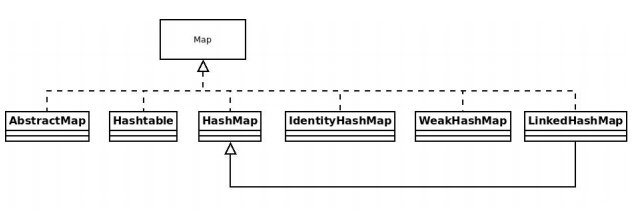
\includegraphics[scale=0.7]{diagramme.jpg}
\end{figure}


Voici les différentes caractéristiques de ces implémentations :
\begin{itemize}
\item AbstractMap : Squelette d'implémentation de Map permettant une réutilisation ultérieure plus facile pour l'utilisateur.
\item HashMap : Permet l'utilisation de clés et valeurs initialisées à null
\item LinkedHashMap : Classe indentique à HashMap si ce n'est qu'elle maintient une double liste contenant toutes les entrées de la HashMap
\item WeakHasMap : Lorsqu'une clé n'est pas utilisée, elle est automatiquement supprimée par le Garbage Collector.
\item IdentityHashMap : Les comparaisons se font par référence (==) et pas par comparaison d'objets (equals).
\end{itemize}

\section*{Question 8 : Kerger Zacharie}

Pour réaliser le retrait d'une entrée d'une table de hachage utilisant la technique du linear probing mais sans marqueur spécial pour représenter les entrées supprimées, il faudrait tout d'abord trouver et supprimer l'élément désiré. Ensuite, on parcourt le tableau (à partir de l'élément supprimé) jusqu'au prochain bucket: s'il est vide, le programme s'arrête, s'il est plein, on supprime l'élément dans le bucket et on le réajoute dans la table de hachage avec une méthode \emph{add(k)} utilisant la technique du linear probing. On recommence cette démarche tant que l'on ne tombe pas sur un bucket vide.\\
\newline
Comme dit précédemment, lorsque l'on supprime un élément, on va ensuite parcourir la table pour supprimer et réajouter tous les éléments présents dans les buckets qui suivent s'ils ne sont pas vides. Par conséquent, dans le pire des cas, on devrait parcourir toute la table de hachage, ce qui équivaudrait à une complexité de O(n). Par contre, en moyenne, la complexité serait plutot de O(1) vu que l'on applique des opérations constantes sur peu d'éléments.



\end{document}
